\subsection{Vista}

La vista contiene los componentes para representar la interfaz del usuario (IU) del programa y las herramientas con las cuales el usuario puede interactuar con los datos de la aplicación. Adicionalmente, la vista se encarga de recibir e interpretar adecuadamente los datos obtenidos del modelo. Cabe mencionar, que al igual que el resto de componentes del MVC, la clase View implementa la interfaz \say{Notify}, la cual permite la comunicación con el resto de elementos.\bigskip

\texttt{loadContent} es el encargado de cargar el contenido inicial en la ventana. Para esta práctica, carga los siguientes elementos semánticos:\bigskip

\texttt{menu}, función que crea y configura el menu de utilidades de la ventana principal. En esta, se incluyen las siguientes opciones: Abrir ventanas de estadísticas, borrado y reseteo de datos, selección de algoritmos, y selección del modo auto.\bigskip

\texttt{body}, función que crea, configura y actualiza la gráfica de la ventana principal. En concreto, se trata de un gráfico de dispersión que contiene el conjunto de puntos de la práctica.\bigskip

\texttt{sidebar}, función que crea y configura la barra de opciones de la derecha de la interfaz principal. Esta permite al usuario interactuar y configurar el entorno de ejecución de los algoritmos.\bigskip

\texttt{footer}, función que crea y configura las opciones de inicio de los algoritmos en la interfaz. Concretamente, este elemento contiene el modo del algoritmo a ejecutar (distancia máxima o distancia mínima) y la opción auto. La opción auto ejecuta los algoritmos seleccionados hasta que no se pueda encontrar ninguna solución más.\bigskip

Adicionalmente, a la vista principal, esta permite desplegar dos ventanas más. Una ventana muestra a tiempo real, el uso y consumo de la memoria de la Java virtual machine (JVM) y la otra ventana muestra las estadísticas de la ejecución de los algoritmos además de su comparación. A continuación, se muestran dos imagenes (\ref{fig:Ejemplo stats JVM} y \ref{fig:Ejemplo stats Algt}) de como se verían las ventanas al iniciarlas junto a una breve explicación de la misma.

\subsubsection{Estadísticas JVM}\label{Stats JVM}

Este apartado de la vista principal, es el encargado de enseñar a tiempo real las estadísticas de la máquina virutal de java. Concretamente, se actualiza cada 0.5s a apartir de los datos obtenidos de la clase de java \say{Runtime} y muestra la memoria libre, la memoria total y el uso de esta en una gráfica de lineas, donde el eje x es instante en el tiempo que se han obtenido los datos y el eje y su valor. Todos los datos de la memoría obtenidos están en MB.

\begin{figure}[!h]
    \centering
    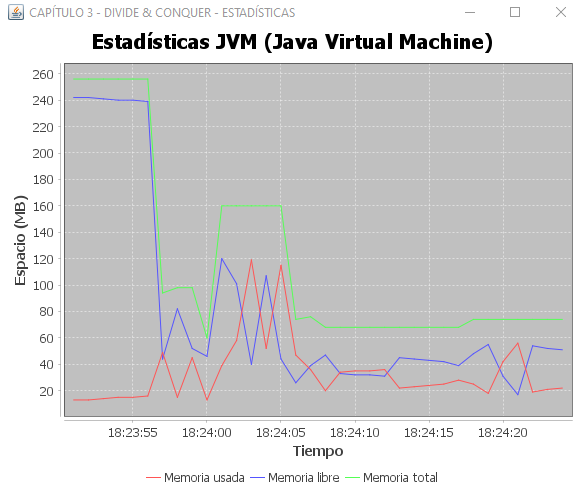
\includegraphics[width=\linewidth]{MVC/View/img/stats-jvm.png}
    \caption{Interfaz estadísticas JVM}
    \label{fig:Ejemplo stats JVM}
\end{figure}

\subsubsection{Estadísticas Algoritmos}\label{Stats Algt}

Este apartado de la vista principal, es el encargado de enseñar las estadísticas de la ejecución de los algoritmos, tanto $N^2$ como $N log N$. Estas estadísticas de cada algoritmo incluyen la media de las distancias, la máxima y mínima distancia y el tiempo medio de ejecución, además de una compración directa entre los algoritmos.

\begin{figure}[!h]
    \centering
    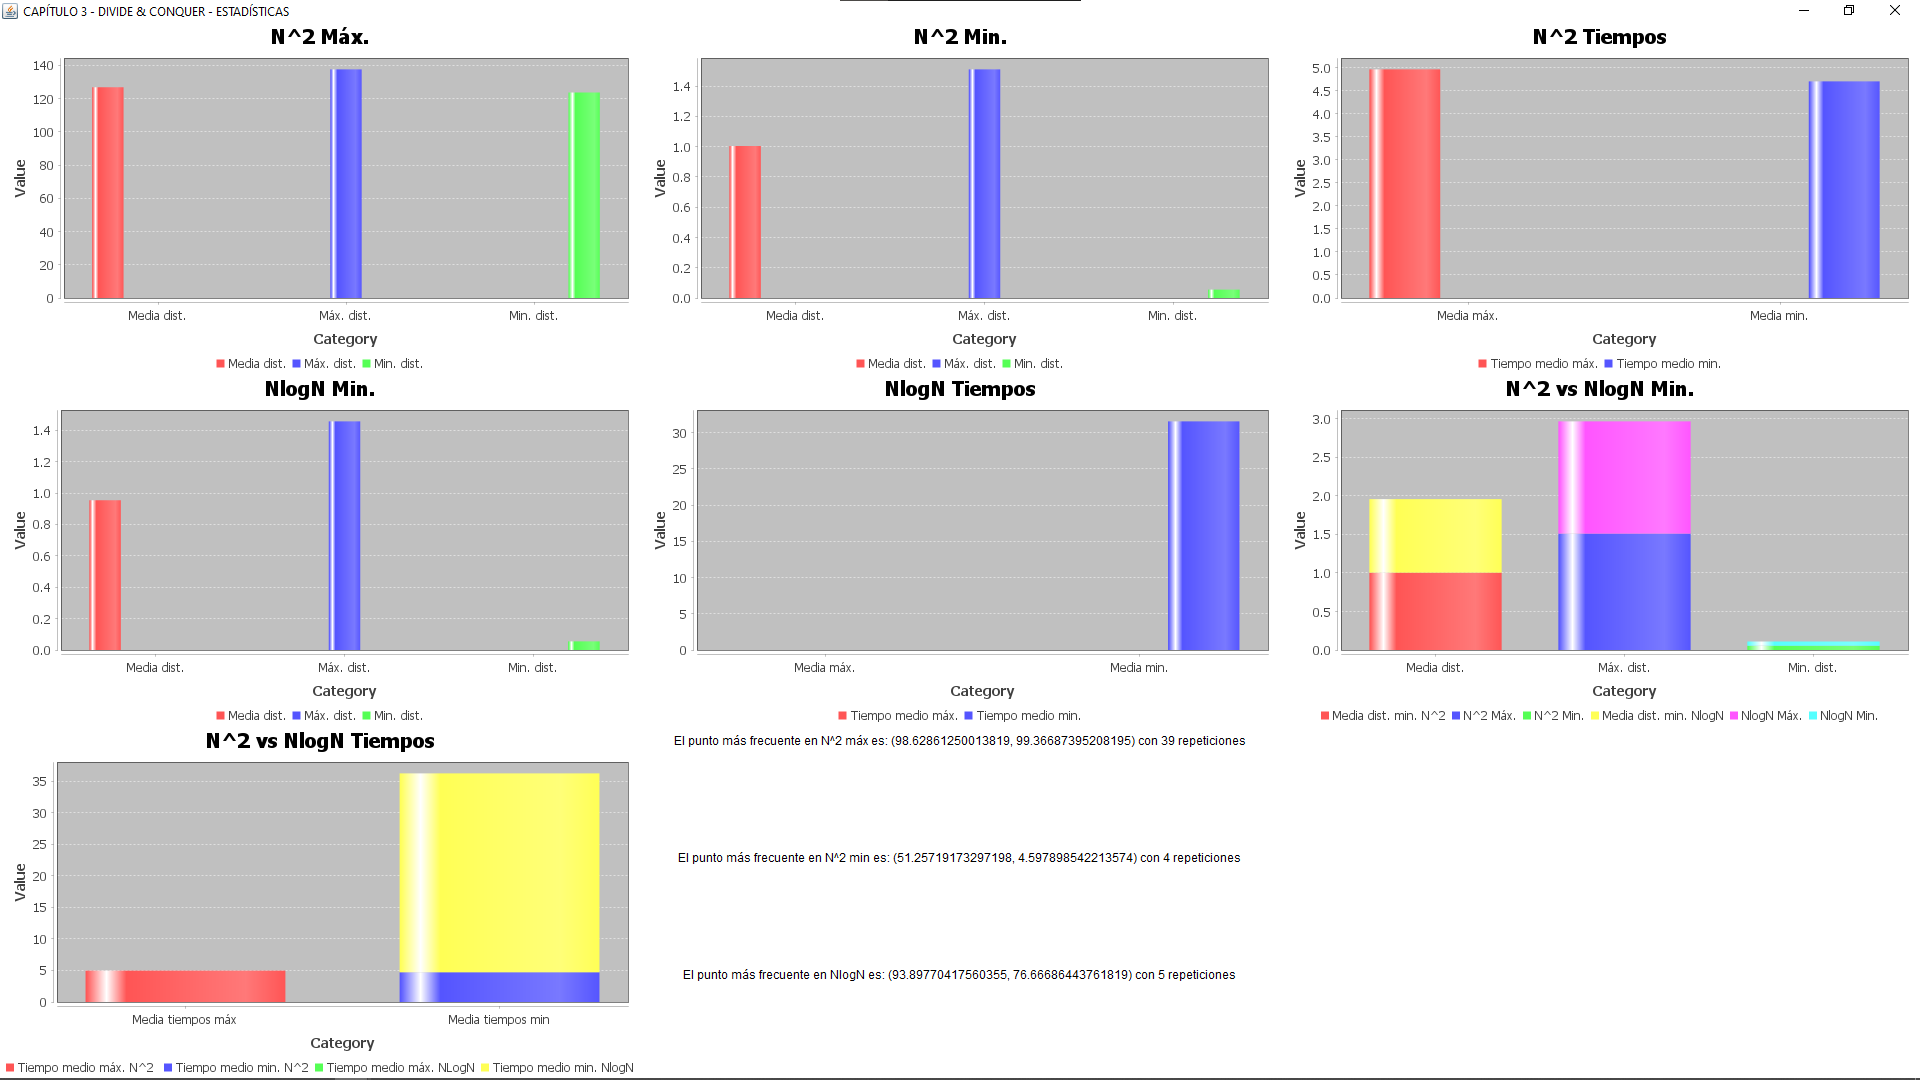
\includegraphics[width=\linewidth]{MVC/View/img/stats-algt.png}
    \caption{Interfaz estadísticas algortimos}
    \label{fig:Ejemplo stats Algt}
\end{figure}

Como se ha podido ver anteriormente en la imagen (\ref{fig:Ejemplo stats Algt}), los datos de las estadísticas están representados con diagramas de barras, donde el eje x es la categoría a la que pertenecen y el eje y el valor correspondiente.
